\section{Introduction}
In genomic analyses, it is commonly of interest to assess whether
there is position enrichment of one set of features near another
\citep{reviewdilemma2014},
or a correlation across samples between nearby genomic features of
different modalities (e.g. gene expression, chromatin accessibility).
For example, enrichment of accessible peaks near sets of genes may
indicate a regulatory relationship \citep{lee2020fluent}, or
enrichment of GWAS fine-mapped variants
near tissue-specific ATAC-seq peaks may suggest
mechanisms of heritability of the GWAS trait.
Such analyses often rely on a null distribution, where one inference
strategy is to permute or shuffle one set of the
genomic features -- giving random positions drawn uniformly along the
genome to existing features, possibly while considering a set of
excluded positions.
Uniformly distributed ``null feature sets'' will not generally exhibit
natural clumping properties of
genomic feature sets, where there often exists a complex
dependency structure.
% both in terms of placement and
% correlation of metadata (signal strength, cell-type-specificity, etc.).
Using an overly simplistic null feature set that doesn't take into
account local dependency of features could result in misleading
conclusions.
Some more sophisticated methods exist, for example
GAT, which allows for controlling feature placement with
respect to local GC content
\citep{GAT_2013}, and regioneR, which implements a ``circular shift'' to
preserve clumping \citep{gel2016regioner}.

The block bootstrap \citep{politis1999subsampling}
provides an alternative to random starts, where one instead generates
random feature sets by sampling large blocks of features from the
original set with replacement, as proposed for features residing in a
segmented genome by \citet{bickel2010subsampling}.
Generating new genomic feature sets via the block bootstrap is more
computationally intensive than a per-feature random start assignment.
To address this, GSC \citep{bickel2010subsampling} implements a
strategy of swapping pairs of blocks in order to generate a bootstrap
distribution while avoiding generation of a genome-scale bootstrap
sample.

Here we describe the \bootranges software, which uses efficient
vectorized code for performing block bootstrap sampling of
\granges \citep{lawrence2013software} objects with the Bioconductor
ecosystem.
\bootranges is part of a modular analysis workflow, where bootstrapped
\granges generated by \bootranges can then be analyzed at block or
genome level using tidy downstream pipelines with \plyranges
\citep{lee2019plyranges}.
Here we demonstrate \bootranges, and additionally provide
recommendations for genome segmentation and block length.
We demonstrate how \bootranges can be incorporated into complex
downstream analyses, for example to avoid arbitrary thresholds when
comparing differentially expressed genes and differentially accessible
peaks.

\vspace*{-20pt}

\section{Features}
\bootranges offers a simple ``unsegmented'' block bootstrap as well as
a ``segmented'' block bootstrap:
since the distribution of features in the genome exhibits multi-scale
structure, we follow the logic of \citet{bickel2010subsampling} and consider to
perform block bootstrapping within \textit{segments} of the genome, which are
more homogeneous in terms of base composition and feature density.
We consider various genome segmentation procedures based on gene
density, or annotations, e.g. Giemsa bands or pre-computed segments
(see software vignette for details).
% Segway segments \citep{hoffman:Segway}, or ChromHMM
% segments\citep{ernst2012chromhmm}),
The genome segments define large (e.g. on the order of ${\sim}1$ MB),
relatively homogeneous segments within which to sample blocks (\cref{fig:framework}A)

The workflow of \bootranges includes downstream analysis with
\plyranges (\cref{fig:framework}B).
The input for the workflow is \granges features \bm{$x$} and
\bm{$y$}, with optional metadata columns (\texttt{mcols}) used for
computing a more complex test statistic than overlap.
Given a segmentation and \texttt{blockLength} $L_b$, a \bootranges
object is generated, which concatenates \granges across bootstrap
iterations. This \bootranges object can be manipulated with \plyranges
to derive the bootstrap distribution of test statistics, and an
empirical p-value.
% the number of times that show an equal or greater statistics than the observed statistic
% or any types of intervals can be reported for testing the null hypothesis that there is no true
% biological relevant association between features.
The \bootranges algorithms are explained schematically in Supplementary \cref{sec:algorithm}.

\vspace{-0.3cm}
\begin{figure}[htbp]
\centering% default with `floatrow`
\setlength{\abovecaptionskip}{-0.05cm}
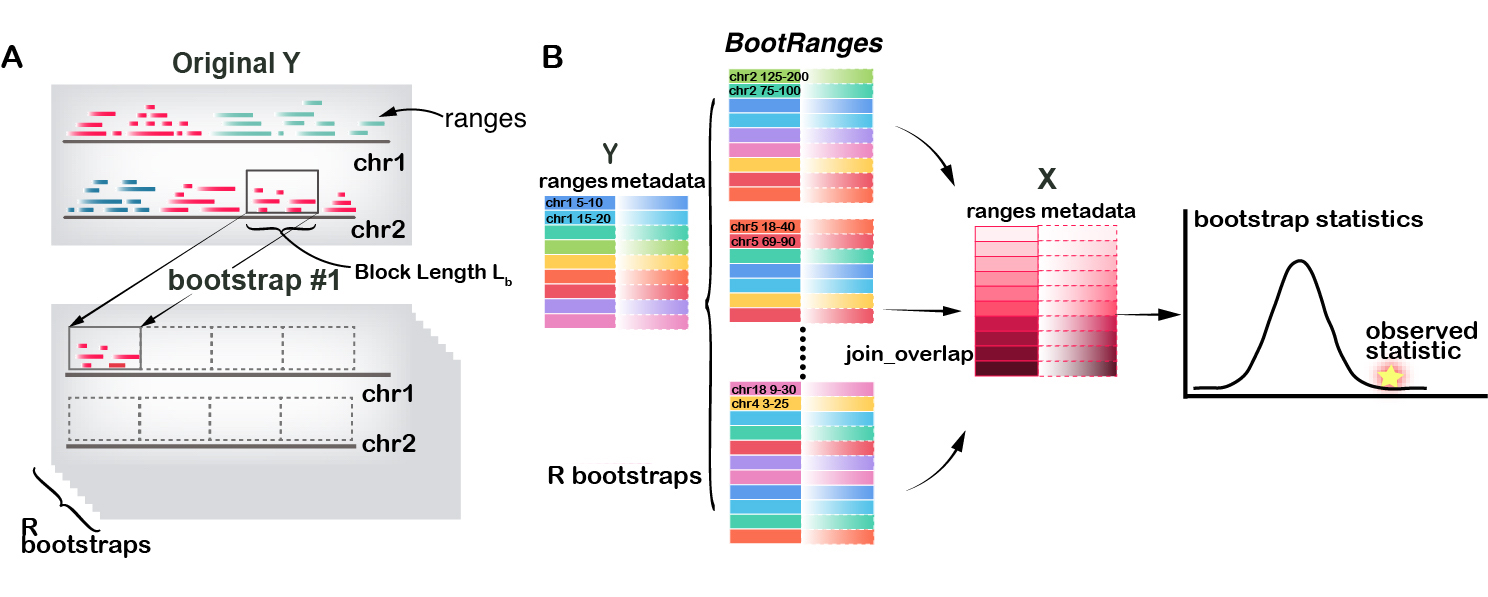
\includegraphics[scale=0.65]{Figures/bootRanges.jpg}
\caption{Overview of \bootranges workflow. (a) A schematic
  diagram of \bootranges with \texttt{blockLength} $L_b$ across chromosome.
  (b) Testing overlaps of features in \bm{$x$} with features in
  \bm{$y$}, and comparing to a null distribution.} 
\label{fig:framework}
\vspace{-0.5cm}
\end{figure}

\vspace*{-20pt}
\section{Application}

First, \bootranges was evaluated on if there was significant overlap
between caQTLs in human liver tissue and SNPs associated with total
cholesterol \citep{CURRIN20211169}.  \cref{fig:result}A shows various
segmentation method and block length effect on overlap rate
distribution. Here overlap rate was defined as the proportion of SNPs
across genome overlapping with peaks within 10kb. The fact that the
estimated statistics variance increase at large $L_b$ indicated data
were inhomogeneous and segmentation
% using either hidden Markov model(HMM) or circular binary search(CBS) \citep{cbs}
could alleviate the scenario. The exceptional decreasing trend using
ChromHMM annotations for Roadmap Epigenomics indicated too many short
segments failed to random swap the block genome when $L_b$ close to
$L_s$.  Regarding the choice of genome segmentation and of block
length selection, we considered a number of diagnostic statistics
including those recommended by \citet{bickel2010subsampling}: the
variance of the null distribution of test statistics
(\cref{fig:result}A) and a scaled version of the change in the width
of the test statistic as $L_b$ changes; as well as examination of the
inter-feature distance distribution (see Supplementary Methods).
After evaluation, $L_b \in [300000,600000]$ was shown to be a good
range for carfully defined null distribution(\cref{fig:suppfig}A-C).
More details were given in Supplementary \cref{sec:results}.

%\vspace{-0.5cm}
\begin{figure}[hbtp]
\centering% default with `floatrow`
\setlength{\abovecaptionskip}{-0.1cm}
\setlength{\belowcaptionskip}{-0.1cm}
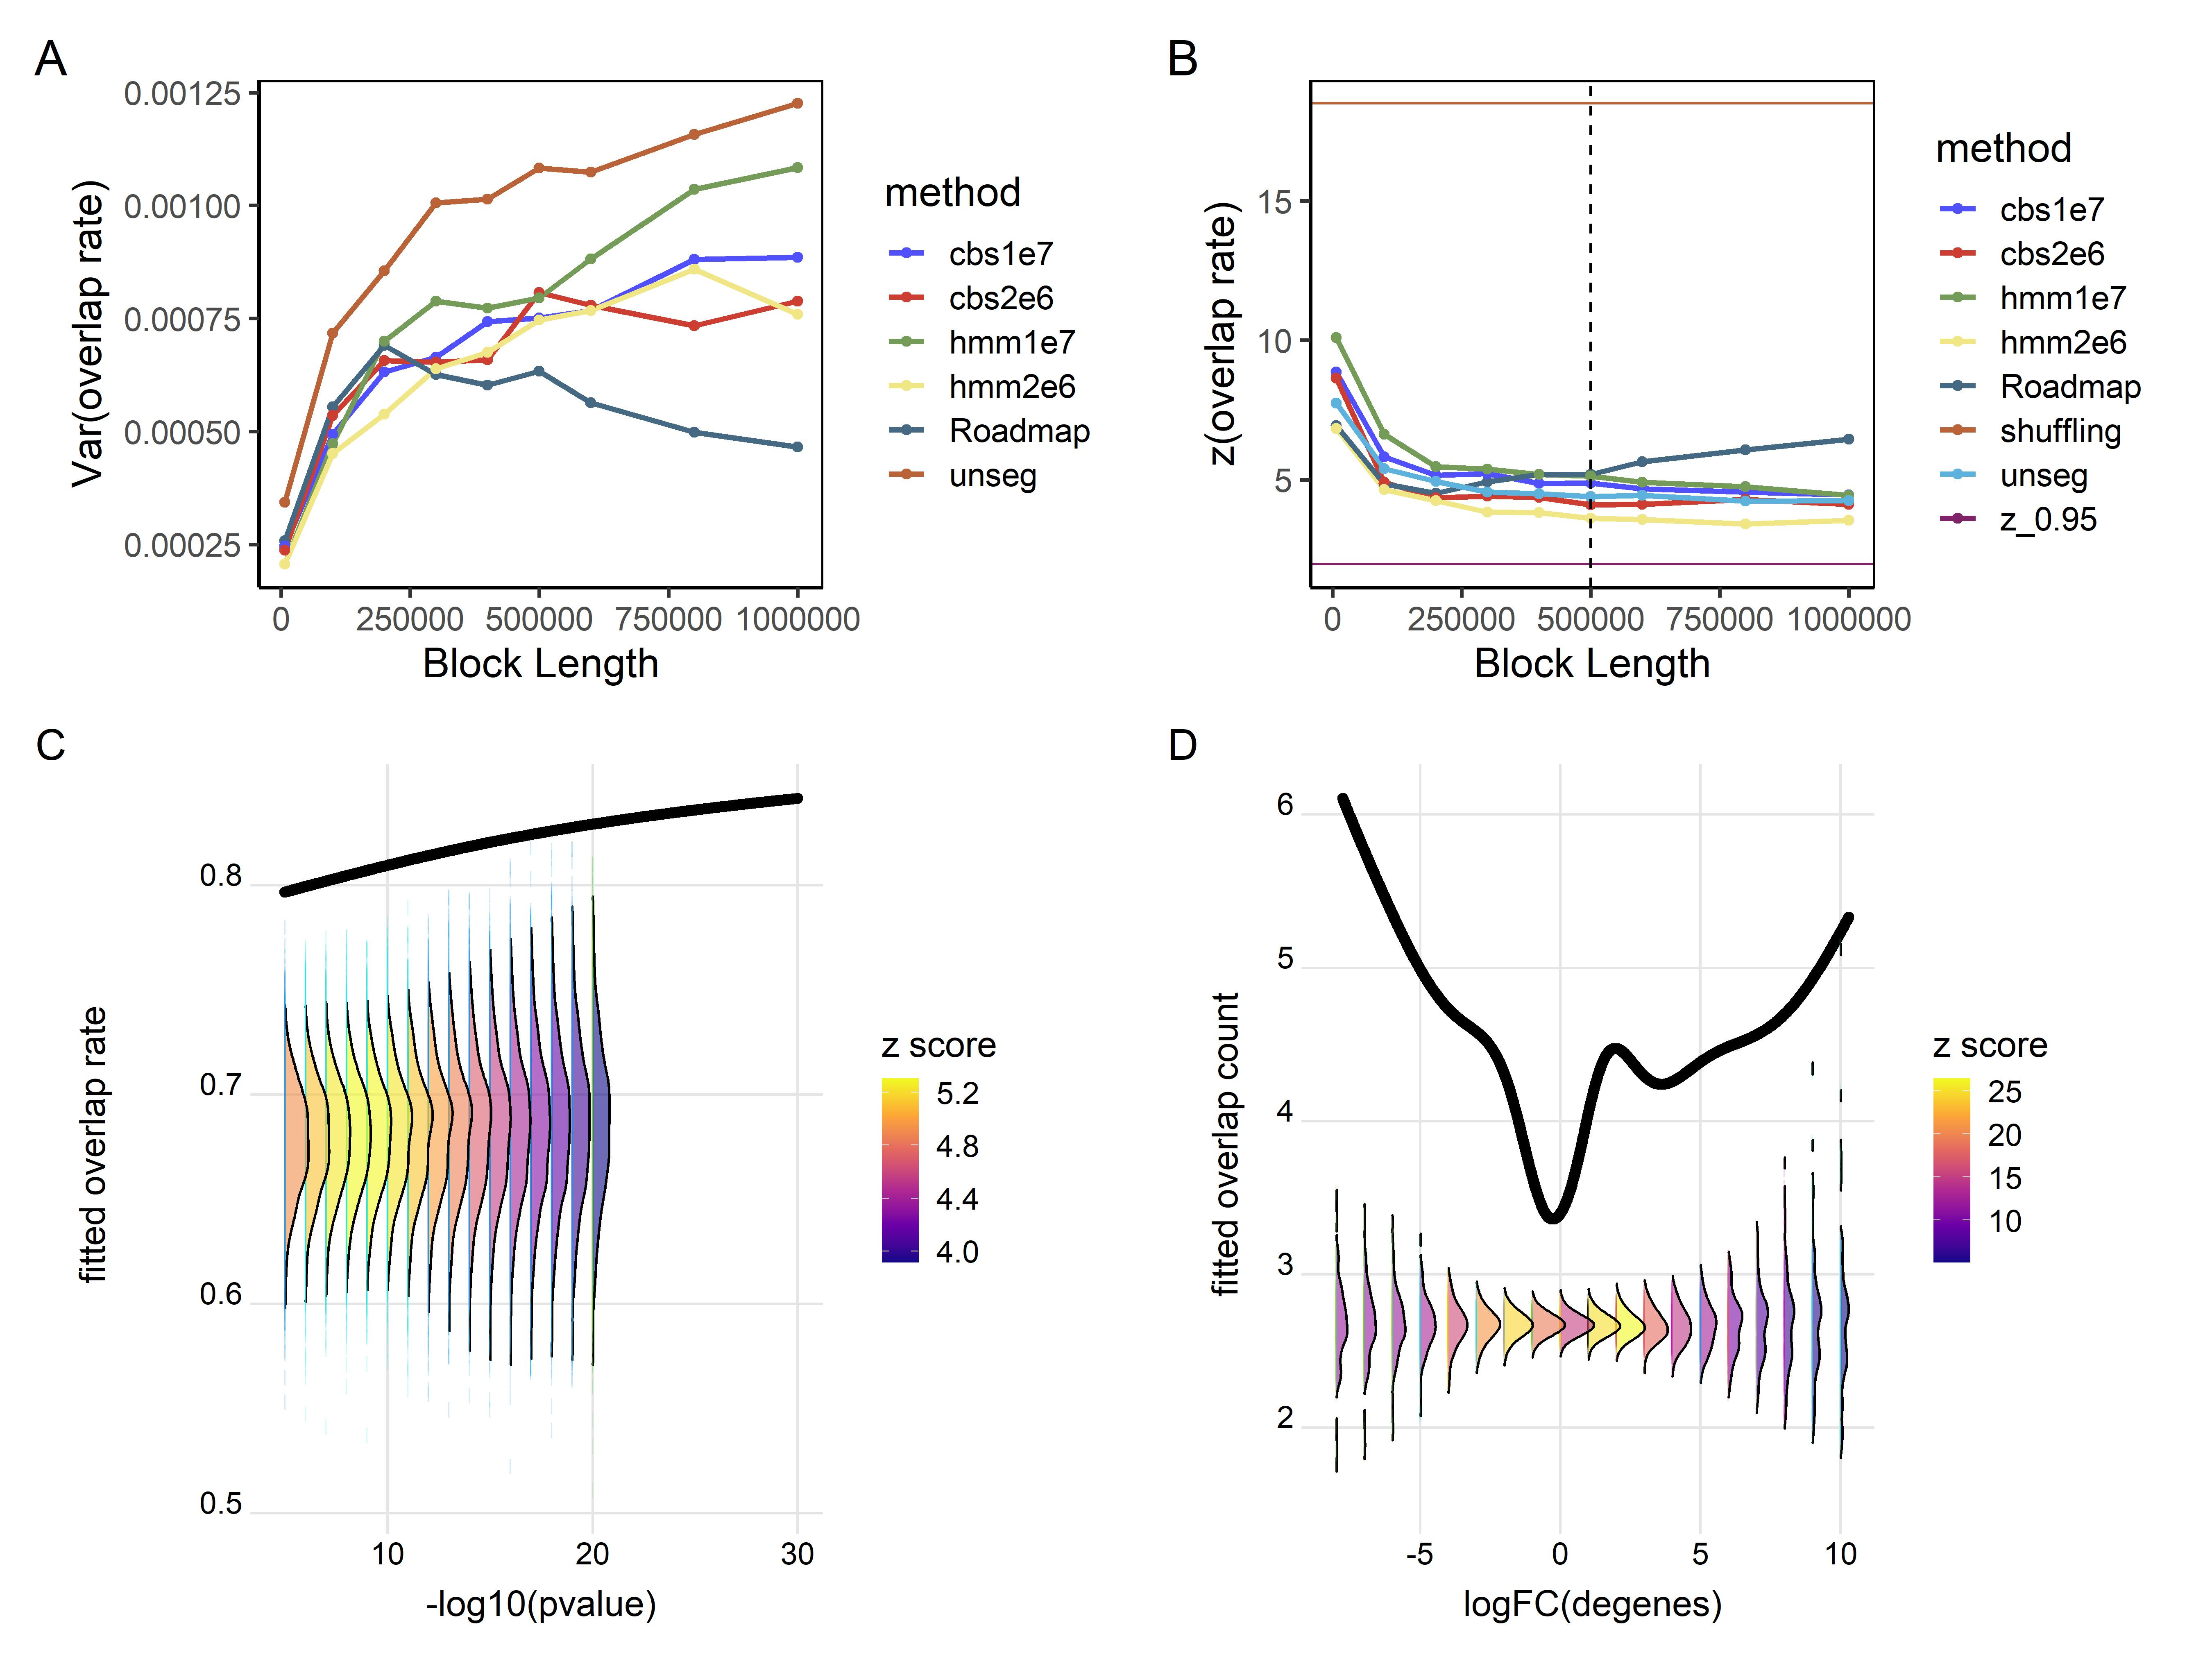
\includegraphics[scale=0.25]{Figures/fig2.jpeg}
\caption{
  Bootstrapping method comparison, and results for enrichment
  analyses. 
  A) Variance of the rate of overlaps
  for various segmentation and $L_b$ combinations (for liver QTL dataset).
  B) $z$ score for the observed overlap
  Upper and lower horizontal line represents the $z$ score obtained
  with naive shuffling and ---.
  C and D) For liver QTL dataset and macrophage dataset, respectively,
  the observed (black line) and bootstrapped (densities) overlap
  seen across various thresholds for GWAS -log10(p-value) (C) and for
  logFC of DE genes (D). Black lines indicate spline fits for the
  observed overlap rate (C) and count (D). The bootstrap conditional
  densities are shown at a grid along the x-axis. Color of density
  represents the $z$ score for the observed overlap statistic.}
\label{fig:result}
\end{figure}

The scientific conclusion of this example was there exists a strong
association between liver caQTLs and total cholesterol SNPs because of
the empirical p value = 0. z score, independent of number of
bootstraps, was used to measure the distance between the expected
value and the observed one according to the standard deviations.
since the the $z = 4.10$ if look at circular binary search(CBS)
\citep{cbs} segmentation method with $L_s = 2e6$ and
$L_b=5e5$(\cref{fig:result}B).  As seen in applications of
\citet{bickel2010subsampling}, the effect of segmentation did not
greatly alter conclusions, e.g. rejection of the null hypothesis, in
this case, although the z score varies greatly among the different
segmentations and block lengths.  Genome shuffling (Supplementary
\cref{sec:shuffle}) that people usually used when performing such
analysis had much higher $z = 18.5$. We believe it may result low
specificity in some cases and block bootstrap was, as much as
possible, close to actual distribution of genomics elements.

In this study, we showed optimized selection of data driven p-value
and logFC through applying \bootranges on pairs of features:
aforementioned example, and chromatin accessibility and gene
expression in a macrophage immune response datasets data
\citep{alasoo2018shared}. A generalized linear model (GLM) with
penalized regression splines from \textit{gam} function in the
\emph{mgcv} R package were fitted and \textit{predict\_gam} function
in the \emph{tidymv} R package were predicted on observed and each
null feature sets.
$$
\setlength{\abovedisplayskip}{3pt}
\setlength{\belowdisplayskip}{3pt}
log \left( \frac{\pi}{1-\pi} \right) = \beta_0  + f (-log_{10}p), log(\mu) = \beta_0 + f (log_{FC})
$$ 
for rate and count-based statistic, separately.  All generated 95\%
percentile intervals at the same time across a range of effect sizes
were displayed by conditional density plot (\cref{fig:result} C,D). We
found z score was highest when -log10(pvalue)=8 (\cref{fig:suppfig}D)
which is quite close to Bonferroni correction and DEG logFC at -2 or
2(\cref{fig:suppfig}E).

We additionally applied \bootranges to Chromium Single Cell Multiome
ATAC + Gene Expression, to assess the correlation of the two
modalities for all pairs of genes and promoter peaks, across the 14
cell types (pseudo-bulk).  For the whole gene set, the mean
correlation of RNA-seq and ATAC log read counts was 0.33 that was
significantly far from the subsampling correlation distribution
(\cref{fig:suppfig}F) with expectation 0.007 and empirical value
indicated there was significant high correlation between genes
expression and open chromatin. Additionally, average gene-promoter
correlation per gene can be derived. XXX of genes have a significant
higher correlation.

According to the time efficiency, we compared with GSC using the
ENCODE kidney and bladder H3K27ac ChIP-seq peaks. The average time to
block bootstrap the whole genome using \bootranges is around 0.3s and
0.37s if adding the \plyranges pipeline. While GSC approximate cost
7.56s. Therefore, \bootranges is 20 times faster.  All of the R code
and data used in this paper are available at the following repository:
\url{https://github.com/Wancen/bootRangespaper}.

\vspace*{-25pt}

\section*{Funding}
This work was funded by CZI EOSS and NIH [NHGRI R01 HG009937]. 
